\begin{figure*}[p]
	\centering
	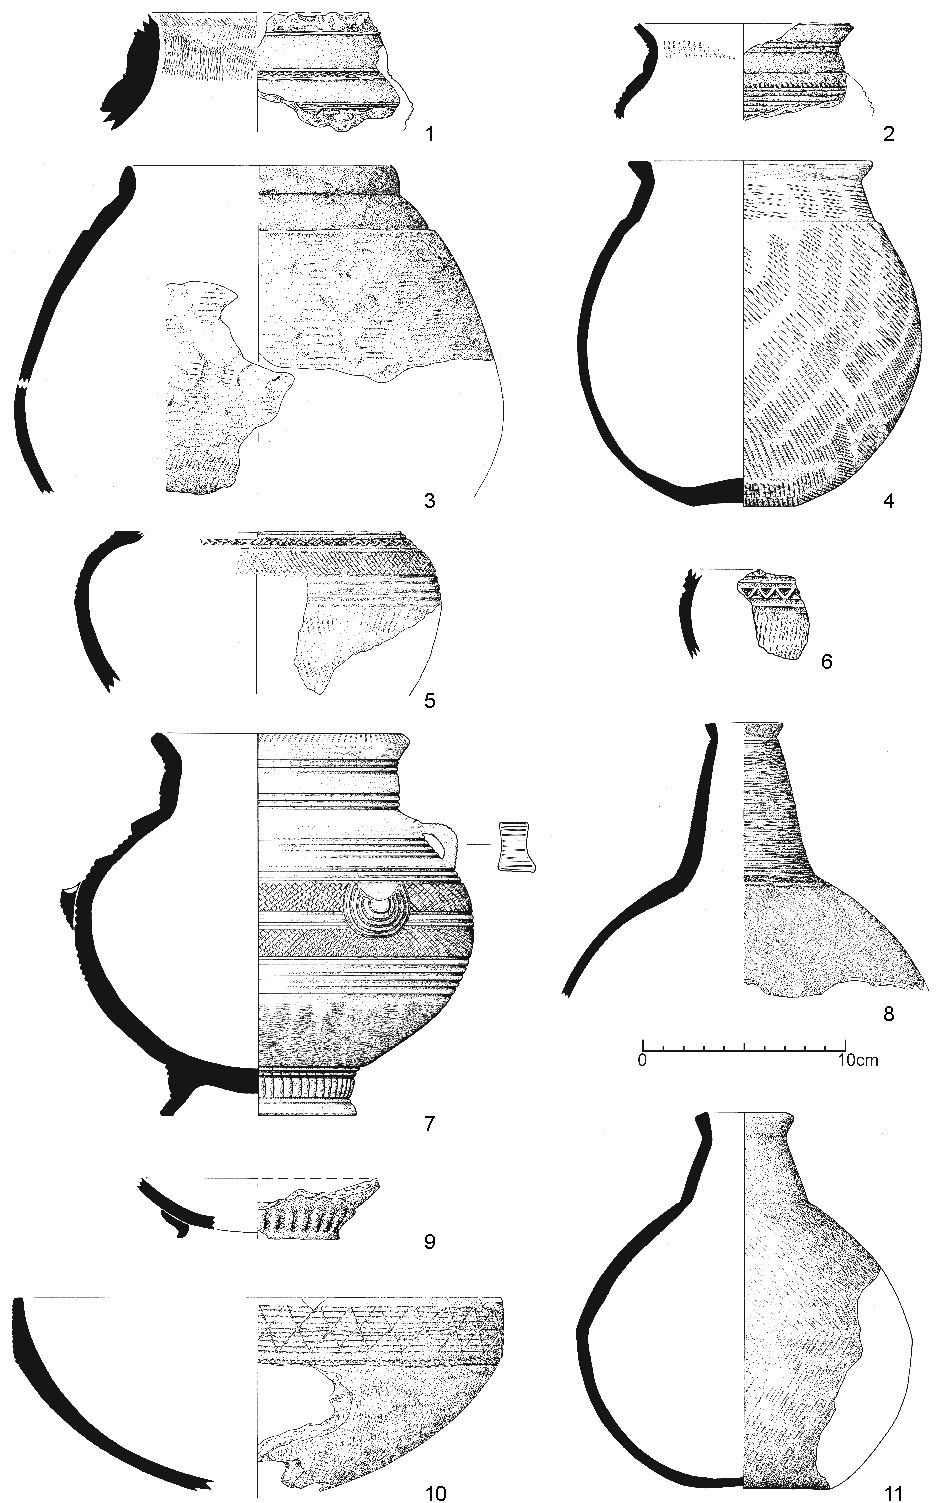
\includegraphics[height = .9\textheight]{fig/EBA-Typen.pdf}
	\caption{Ebambe-Gruppe: Typvertreter.\\1:~Taf.~55.4; 2:~Taf.~54.15; 3:~Taf.~41.9; 4:~Taf.~89.4; 5:~Taf.~49.16; 6:~Taf.~55.8; 7:~Taf.~56.15; 8:~Taf.~82.9; 9:~Taf.~62.14; 10:~Taf.~82.4; 11:~Taf.~90.1.}
	\label{fig:EBA_Typvertreter}
\end{figure*}

\begin{figure*}[tb]
	\begin{minipage}[b]{\columnwidth}
		\includegraphics[width=\textwidth]{fig/BYN87-101_Gef_aus_Epena_E87-023-10.jpg}
	\end{minipage}\hfill
	\begin{minipage}[b]{\columnwidth}
		\caption{Ebambe-Gruppe: Flasche vom Typ A2 der Ebambe-Gruppe in Boyenge am Unterlauf des \mbox{Likwala}-\mbox{aux}-\mbox{Herbes} (Fpl.~284). Der Gefäßkörper ist mit flächigem \textit{banfwa-nfwa} (Tab.~\ref{tab:Verzierungselemente}: 08) verziert, während der Hals horizontale, feine Rillen (Tab.~\ref{tab:Verzierungselemente}: 02.1) sowie diagonal gestellte Eindrücke (Tab.~\ref{tab:Verzierungselemente}: 04.12) aufweist. Nach Angabe der lokalen Bevölkerung stammt das Gefäß aus Epena (Fpl.~306), wo entsprechende Formen seinerzeit noch getöpfert worden sein sollen (Foto: M. K. H. Eggert, 1987).}\label{fig:EBA_BoyengeE8702310}
	\end{minipage}
\end{figure*}

\subsubsection{Ebambe-Gruppe}\label{sec:EBA-Gr}

Die Ebambe-Gruppe, benannt nach einer Fundstelle am mittleren \mbox{Likwala}-\mbox{aux}-\mbox{Herbes} (Fpl.~297), beschreibt eine vor allem entlang des \mbox{Sangha} und \mbox{Likwala}-\mbox{aux}-\mbox{Herbes} verbreitete Keramik, die enge Beziehungen zur rezenten Epena-Keramik (Kap.~\ref{sec:EPE-Gr}) sowie Ähnlichkeiten zu Stilgruppen des Inneren Kongobeckens aufweist (Tab.~\ref{tab:EBA_VglICB}). Die chronologische Stellung des Stils lässt sich nicht genauer als auf das 2.~Jt. n.~Chr. eingrenzen (siehe unten). Insgesamt umfasst die Ebambe-Gruppe 280~GE. Weitere 520 Einzelscherben ließen sich nur unter Vorbehalt und aufgrund einzelner Merkmale zuweisen: dazu zählen vor allem Stücke mit der nur bei dieser Stilgruppe in diesem Maße beobachteten, flächigen \textit{banfwa-nfwa}-Verzierung. Aufgrund der starken Fragmentierung der Stücke und da es sich größtenteils um ansonsten wenig diagnostische Wandungsfragmente handelte, wurden sie lediglich ausgezählt.\footnote{91\,\% der 520 ausgezählten Stücke sind Fragmente der Gefäßwandung, während es sich bei 7\,\% um Rand- und bei 2\,\% um Bodenstücke handelt. Ausgezählt wurden Teile der Inventare von 13 der insgesamt 32 Fundstellen der Ebambe-Gruppe. Vornehmlich wurden Teile der Inventare der Ausgrabung MUN~87/1 (Kat.-Nr.~15; n=291) in Munda (Fpl.~304) sowie PIK~87/2 (Kat.-Nr.~9; n=83) in Pikunda (Fpl.~255) ausgezählt. Zudem wurden größere Teile der Surveyfunde aus Ebambe (Fpl.~297; n=39) und Mosenge (Fpl.~299; n=55) ausgezählt. Alle übrigen Inventare übersteigen zehn ausgezählte Scherben nicht.} 66\,\% aller der Ebambe-Gruppe zuordneten Scherben wurden als sicher der Stilgruppe zugehörig angesprochen. Keramik des Ebambe-Stils wurde an 32 Fundstellen entlang des \mbox{Sangha} und \mbox{Likwala}-\mbox{aux}-\mbox{Herbes} sowie an je einer Fundstelle am \mbox{Ngoko}, Kongo und \mbox{Ubangi} angetroffen (Abb.~\ref{fig:EBA_Verbreitung}). Über die Hälfte aller Funde (57\,\%) stammen aus zwei Grabungen in Pikunda am mittleren \mbox{Sangha} (Fpl.~255) sowie in Munda am oberen \mbox{Likwala}-\mbox{aux}-\mbox{Herbes} (Fpl.~304).\footnote{Das Inventar aus dem Befund MUN~87/1 wurde als definierender Komplex für die Beschreibung der keramischen Variabilität der Stilgruppe herangezogen.} Die Surveyfunde spiegeln die diagnostischen Eigenschaften der Stilgruppe in gleichem Maße, wenn nicht sogar noch stärker als die Grabungsfunde wider.\footnote{Mit Blick auf die Fragmentierung von Grabungs- und Surveyfunden ergeben sich zwischen den anteiligen Häufigkeiten der jeweiligen Größenklassen keine Unterschiede. Während der Anteil stark bis mittelstark zerscherbter Stücke bei der Grabungsfunden höher ist, zeichnen sich die Surveyfunde sogar durch eher etwas größere Fragmente sowie kaum fein zerscherbtes Material aus. 73\,\% aller Grabungsfunde sind kleiner als 70\,$\times$\,70\,mm, während es bei den Surveyfunden lediglich 33\,\% sind. Etwa 13\,\% der Surveyfunde sind größer als 120\,$\times$\,120\,mm, während es bei den Grabungen nur 7\,\% sind.} Das Inventar der Stilgruppe besteht aus etwa 76\,\% Wandungsscherben. Lediglich 18\,\% aller Stücke sind Randfragmente und 4\,\% Bodenstücke. Ebenfalls wurden zehn vollständige oder hinreichend vollständige Gefäße der Stilgruppe zugewiesen.

\paragraph{Technologische Merkmale}\hspace{-.5em}|\hspace{.5em}%
Die der Ebambe-Gruppe zugewiesenen GE weisen fast ausschließlich die \textit{Fabrics} 1 beziehungsweise 2 auf (94\,\%), die praktisch keine nichtplastischen Partikel enthalten.\footnote{Die \textit{Fabrics} 3a--c, 4a, 7d, 8a sowie 9a--b bilden die deutliche  Ausnahme und fanden sich lediglich an sechs Fundstellen am mittleren und oberen \mbox{Sangha}: Pikunda (Fpl.~255), Molanda (Fpl.~258), Mosanya (Fpl.~262), Ouesso (Fpl.~265), Maboko (Fpl.~267) und Mai~mpembe (Fpl.~271) sowie in Mbenja (Fpl.~277) am \mbox{Ngoko}.} Die Scherben enthalten regelhaft weniger als 1--2\,\% (74\,\%) beziehungsweise 3--5\,\% nichtplastische Partikel (18\,\%), die sich vornehmlich den Größenklassen \textit{very fine} bis \textit{medium} (zusammen 92\,\%) zurechnen lassen. Lassen sich nichtplastische Partikel beobachten, handelt es sich fast ausnahmslos um Quarz, der in heterogenen, verrundeten und sehr feinen Korngrößen vorkommt. Es kann daher davon ausgegangen werden, dass es sich bei den beobachteten Partikeln nicht um dezidierte Zusätze im Sinne einer intentionellen Magerung des Tones handelt, sondern um Partikel, die natürlich in den genutzten Tonen vorkommen. Der Großteil der GE spricht für eine -- aus der Färbung der Scherben abgeleitete -- Nutzung weißbrennender Tone (67\,\%). Lediglich 8\,\% aller Scherben deuten auf die Nutzung rotbrennender Tone hin, während sich schwarz, grau oder beige gefärbte Stücke (25\,\%) einer Ansprache der Brennfarbe der Tone entzogen. Die Oberflächen sind regelhaft glatt (93\,\%) oder nur leicht rau (5\,\%).
%Die Wandungen sind im Mittel 6,4\,mm dick, bei einer Varianz von 3,4\,mm.

\begin{table*}[!tb]
	\centering
	{\footnotesize \begin{sftabular}{@{}lcc|cccc@{}}
			\toprule
			& \textbf{EBA} & \textbf{EPE} & \textbf{MBA} & \textbf{BDG} & \textbf{NKI} & \textbf{BOT} \\
			\midrule
			Flasche mit geschweifter Wandung (A2) & $\bullet$ & & & & & $\bullet$ \\
			Flasche mit profilierter Wandung (A3) & & $\bullet$ & & & & \\
			Hohes Gefäß mit Kegelhals (B4) & $\bullet$ & $\bullet$ & & & & \\
			Hohe Gefäße B2--3 & & $\bullet$ & & & & \\
			Gefäße mit geschweifter Wandung (E/D) & & & $\bullet$ & $\bullet$ & $\bullet$ & $\bullet$ \\  \hdashline[0.5pt/5pt]
			Schulterabsatz \& Kegelhals & $\bullet$ & & $\circ$ & $\bullet$ & $\bullet$ & \\
			Böden mit konkaver Standfläche (B6) & $\bullet$ & $\bullet$ & & & & \\
			\textit{banfwa-nfwa}-Verzierungen & $\bullet$ & & $\bullet$ & $\bullet$ & $\bullet$ & $\bullet$ \\
			\bottomrule
	\end{sftabular}}
	\caption{Ebambe-Gruppe: Gemeinsamkeiten mit der Stilgruppe Epena sowie potenziell zeitgleichen Gruppen des Inneren Kongobeckens.\\$\bullet$ vorhanden, $\circ$ fraglich. \\ EBA: Ebambe, EPE: Epena (Kap.~\ref{sec:EPE-Gr}), MBA: Mbandaka \parencite[139--143]{Wotzka.1995} , BDG: Bondongo \parencite[128--139]{Wotzka.1995}, NKI: Nkile \parencite[144--150]{Wotzka.1995}, BOT: Botendo \parencite[150--158]{Wotzka.1995}.}
	\label{tab:EBA_VglICB}
\end{table*}

\paragraph{Formen}\hspace{-.5em}|\hspace{.5em}%
Die Gefäßmorphologie der Ebambe-Gruppe ließ sich bei insgesamt 203~GE beobachten. Das Gefäßformen-Spektrum umfasst fast ausschließlich hohe Gefäße (Typ~B), schalenförmige Gefäße mit abknickender Wandung (Typ~G) sowie flaschenförmige Gefäße (Typ~A). Bei 62\,\% aller GE war eine sichere Zuweisung des Gefäßtyps möglich. Die charakteristische und auch diagnostische Gefäßform des Ebambe-Stils sind hohe Gefäße mit einem Schulterabsatz und teilweise kurzem Kegelhals vom Typ B4. Diese machen 57\,\% aller sicher zugewiesenen GE aus (Abb.~\ref{fig:EBA_Typvertreter}.3--4). Ebenfalls häufig finden sich schalenförmige Gefäße mit einem leicht konvexen Gefäßunterteil, einer abknickenden Wandung und einem geraden, zylindrischen Oberteil vom Typ G4 (23\,\%; Abb.~\ref{fig:EBA_Typvertreter}.10). Flaschenförmige Gefäße (Typ~A) machen 11\,\% der GE aus (Abb.~\ref{fig:EBA_Typvertreter}.8,11; Abb.~\ref{fig:EBA_BoyengeE8702310}). Die Ränder werden von kurzen, einfach ausbiegenden (B1; 46\,\%; Abb.~\ref{fig:EBA_Typvertreter}.2,4,7,8,11) sowie parallel aufsteigenden Formen (A1; 34\,\%; Abb.~\ref{fig:EBA_Typvertreter}.3,10) bestimmt. An 83\,\% aller GE, bei denen die Halspartie erhalten war, konnte ein häufig kurzer Kegelhals beobachtet werden (Abb.~\ref{fig:EBA_Typvertreter}.1--4). Unterhalb dieses Kegelhalses findet sich bei 73\,\% ein getreppter Schulterabsatz, der in der Hälfte aller Fälle nur 1--2\,mm breit ist (Abb.~\ref{fig:EBA_Typvertreter}.3--5). Bei 31~GE ließ sich die Form des Gefäßbodens beobachten. Das Gros sind flache Böden mit konkaver Standfläche vom Typ B6 (42\,\%; Abb.~\ref{fig:EBA_Typvertreter}.10; Taf.~83.5) sowie einfache, flache Standböden (B4; 29\,\%; Abb.~\ref{fig:EBA_Typvertreter}.4; Taf.~88.7, 89.7). Böden mit einem Standring, der häufig vertikal verlaufende Einkerbungen aufweist, machen 13\,\% der Bodenstücke aus (B13; Abb.~\ref{fig:EBA_Typvertreter}.7,9; Taf.~88.8). In 16\,\% der Fälle zeigten sich runde Böden (B1--2; Taf.~71.4).

\paragraph{Verzierungen}\hspace{-.5em}|\hspace{.5em}%
Die Gefäße der Ebambe-Gruppe weisen regelhaft flächige \textit{banfwa-nfwa}-Verzierungen auf. Diese machen insgesamt 35\,\% aller beobachteten Verzierungselemente aus und finden sich vornehmlich auf dem Gefäßbauch sowie Bodenansatz (Anlage~4\subref{fig:EBA_Verz}). Des Weiteren ist die Ebambe-Keramik durch Riefen- und Rillen (Tab.~\ref{tab:Verzierungselemente}: 01--02) bestimmt; zusammen 47\,\% aller Verzierungselemente. Die häufigste Variante sind horizontale Rillen, die 26\,\% aller aufgenommenen Verzierungselemente ausmachen und die vor allem außen am Rand sowie im Bereich der Gefäßhälse und Gefäßschultern zu beobachten sind (Anlage~4\subref{fig:EBA_Verz}). Auf den Gefäßschultern finden sich zudem Reihen diagonal gesetzter (Tab.~\ref{tab:Verzierungselemente}: 04.12; 8\,\%) sowie lange bogenförmige Eindrücke (Tab.~\ref{tab:Verzierungselemente}: 04.19; 3\,\%). \textit{Schachbrett}-Muster aus diagonalen, feinen Rillen (Tab.~\ref{tab:Verzierungselemente}: 01.2; 5\,\%) sowie mit Rillen gefüllte Flächen (Tab.~\ref{tab:Verzierungselemente}: 1.8, 3\,\%) können ebenfalls auf den Oberteilen der Gefäße beobachtet werden. Die flächige Verzierung der Gefäßunterseiten mit \textit{banfwa-nfwa} einerseits und der Oberteile und Hals- sowie Randbereiche mit Riefen, Rillen und Eindrücken andererseits erinnert an die Verzierungspraxis der Botendo-Gruppe (\textsc{Wotzka} 1995: 150--158, Taf.~48.3,9, Taf.~49.1). Die Nutzung von \textit{banfwa-nfwa} ist eines der bestimmenden Charakteristika für die Abgrenzung der Ebambe-Keramik zur Epena-Gruppe (Kap.~\ref{sec:EPE-Gr}), deren Gefäße praktisch kein \textit{banfwa-nfwa} zeigen (Anlage~4\subref{fig:EPE_Verz}). 

\paragraph{Datierung}\hspace{-.5em}|\hspace{.5em}%
Die chronologische Ansprache der Ebambe-Keramik muss anhand mehrerer unabhängiger Quellen diskutiert werden: aus Munda am \mbox{Likwala}-\mbox{aux}-\mbox{Herbes} sowie Pikunda am \mbox{Sangha} vorliegenden Radiokohlenstoffdatierungen, zwei ethnografischen Belegen und morphologische wie ornamentale Ähnlichkeiten zu anderen keramischen Stilgruppen im Arbeitsgebiet sowie dem Inneren Kongobecken. Die Beschreibung der Ebambe-Gruppe geht vor allem auf das Inventar der Grabung MUN~87/1 in Munda am \mbox{Likwala}-\mbox{aux}-\mbox{Herbes} (Kat.-Nr.~12) zurück. Die Grabung erbrachte einen aus zwei Teilen bestehenden Befund, einen flachen, kleinen Verhüttungsbefund, der sich an eine größere Grube anschließt. Aus beiden Teilen liegen Radiokohlenstoffdatierungen vor. Zwei Datierungen aus dem Verhüttungsbefund fallen in das 7.--14.~Jh. n.~Chr. (Tab.~\ref{tab:MUN87-1_14C-Daten}: KI-2882, KI-2883) und eine Datierung aus der größeren, ausschließlich Keramik der Ebambe-Gruppe enthaltenden Grube datiert jünger als das 16.~Jh.~n.~Chr (KI-2884). Die stratigraphischen Beobachtungen bei der Grabung weisen jedoch auf die Grube als den älteren Befundteil hin (siehe Kat.-Nr.~12). Eine Besonderheit der Befundsituation in Munda ist, dass sich in der direkt an den Verhüttungsbefund anschließenden Grube kaum Schlacken fanden, sich also kein funktionaler Zusammenhang zwischen den beiden Teilen ergibt.\footnote{Anders als etwa bei einem 2015 in Iyonda, südlich von Mbandaka am Kongo ausgegrabenen Verhüttungsbefund. Dieser, ein offener Ofen wie jene, die Anfang der 1980er Jahre in Bamanya durch das \textit{River Reconnaissance Project} untersucht wurden \parencite[3235--3237]{Eggert.1987}, besteht aus einem flachen Verhüttungsofen mit seitlichem Schlackenabfluss, der in eine im unteren Bereich mit Fließschlacken verfüllte Grube ableitete \parencite{Jungnickel.2016}.} Der stratigraphische Befund, demzufolge die Verfüllung der Grube durch den Verhüttungsbefund geschnitten und überlagert werden soll, wurde lediglich in einem sehr begrenzten Bereich beobachtet (Abb.~\ref{fig:MUN87-1_Querprofil_Zeichnung+Foto}). Ein weiteres, mit Keramik der Ebambe-Gruppe (Abb.~\ref{fig:EBA_Typvertreter}.5) assoziiertes Radiokohlenstoffdatum aus dem Verhüttungsbefund PIK~87/3 in Pikunda am \mbox{Sangha} (Kat.-Nr.~10) fällt in das 11.--13.~Jh. n.~Chr. (KI-2892).\footnote{Da leider keine Dokumentation zu dieser Grabung vorliegt, lassen sich die stratigraphischen und räumlichen Bezüge zwischen Befundsituation, gemachten Funden und der zugehörigen Radiokohlenstoffdatierung nicht mehr rekonstruieren. Siehe Kat.-Nr.~10.}

\begin{figure*}[p]
	\centering
	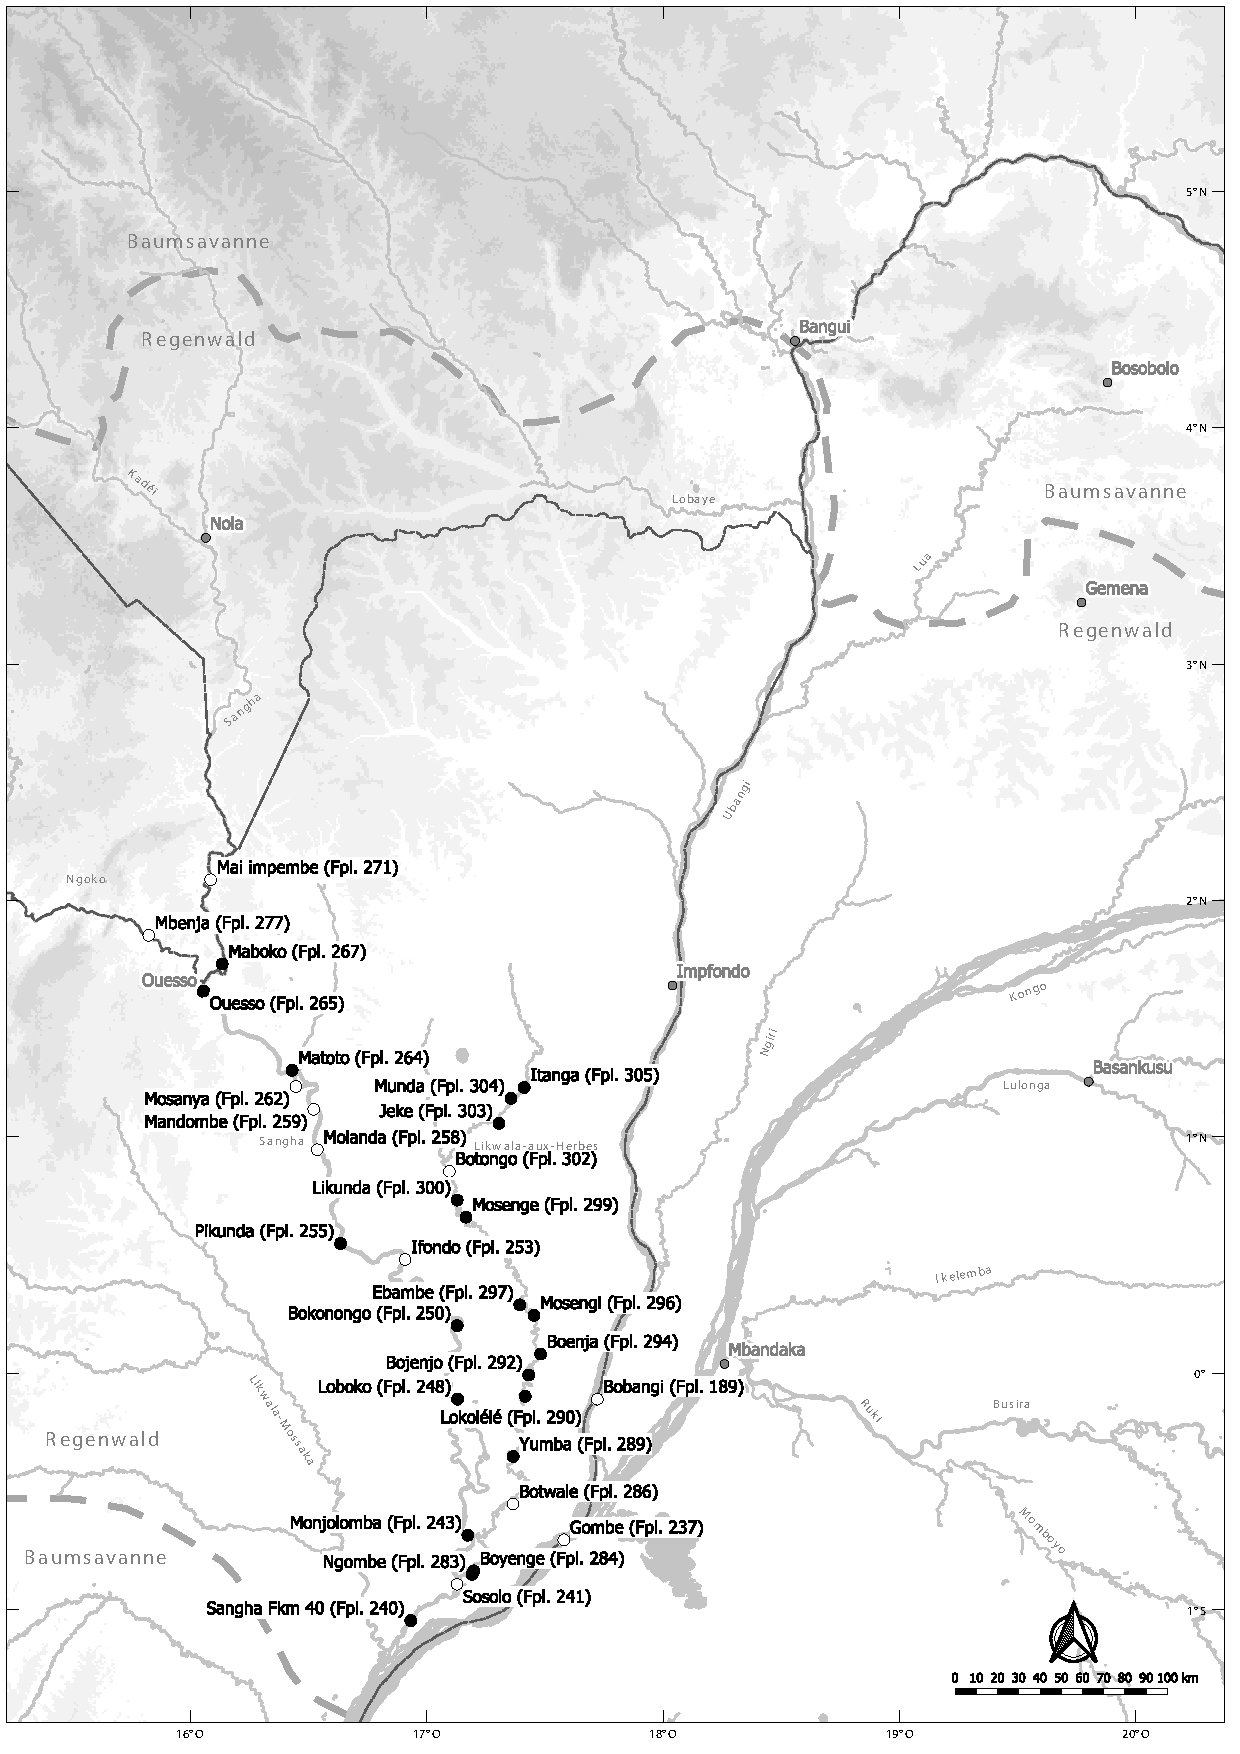
\includegraphics[width=\textwidth]{fig/EBA_Verbreitung.pdf}
	\caption{Ebambe-Gruppe: Verbreitung.}
	\label{fig:EBA_Verbreitung}
\end{figure*}

Ein diesen Datierungen entgegen laufendes aber starkes chronologisches Indiz stellt die Beobachtung einer Flasche der Ebambe-Gruppe in Boyenge (Fpl.~284) am unteren \mbox{Likwala}-\mbox{aux}-\mbox{Herbes} dar, die 1987 noch in Benutzung war und aus Epena (Fpl.~306) stammen soll (Abb.~\ref{fig:EBA_BoyengeE8702310}). Auch die in Boleko am unteren \mbox{Likwala}-\mbox{aux}-\mbox{Herbes} beobachtete Töpferin stellt eine Flasche her, die morphologisch der Keramik der Ebambe-Gruppe entspricht.\footnote{Siehe Anm.~\ref{ftn:EthnoToepfereiInVorb}.} Diese beiden Belege deuten ein rezentes Alter der Ebambe-Keramik an.

Mit Blick auf die formalen Ähnlichkeiten zu anderen Stilgruppen des Arbeitsgebiets sind vor allem die starken Parallelen zur rezenten Epena-Keramik zu nennen (Kap.~\ref{sec:EPE-Gr}). Beiden Stilgruppen gemein sind hohe Gefäße mit kurzem Kegelhals und schmalem Schulterabsatz vom Typ B4. Die größten Unterschiede zwischen den beiden Gruppen sind das ausschließliche Auftreten von Flaschen mit geschweifter Wandung vom Typ A2 innerhalb des Ebambe-Stils, während die Epena-Gruppe durch Flaschen mit deutlich profilierter Wandung und breitem Schulterabsatz vom Typ A3 bestimmt wird. Auch die hohen Gefäße mit weiter Mündung vom Typ B2--3, die Teil des Epena-Stils sind, finden sich im Material der Ebambe-Gruppe nicht. Das in vielen Fällen für die Ansprache der Stücke diagnostische Merkmal ist jedoch das Fehlen von \textit{banfwa-nfwa} innerhalb der Epena-Gruppe, die für die Ebambe-Keramik das bestimmende Verzierungselement darstellt. Schmale Schulterabsätze und ein kurzer Kegelhals, wie sie innerhalb der Ebambe-Keramik beobachtet werden können, finden sich auch bei der mindestens in das 13.--14.~Jh. n.~Chr. datierenden Nkile-Gruppe des Inneren Kongobeckens \parencite[144--150]{Wotzka.1995}. 

In der Zusammenschau betrachtet deuten die vorgebrachten Quellen eher auf ein subrezentes bis rezentes Alter der innerhalb der Ebambe-Gruppe zusammengefassten keramischen Formen hin. Jedoch können beim gegenwärtig sehr schwachen Quellenstand die beiden in das 7.--14.~Jh. n.~Chr. fallenden Radiokohlenstoffdatierungen aus MUN~87/1 in Munda (KI-2882, KI-2883) sowie das eine, ins 11.--13.~Jh. n.~Chr. gehörige Datum aus PIK~87/3 in Pikunda (KI-2892) nicht vollkommen außer Acht gelassen werden, die zudem durch lose Parallelen zur Nkile-Keramik des Inneren Kongobeckens unterstützt werden. Abschließend muss konstatiert werden, dass sich zum ersten Auftreten der Ebambe-Keramik im Arbeitsgebiet gegenwärtig keine belastbaren Angaben machen lassen, dass sie jedoch bis in rezente Zeit in Benutzung war, ist hinreichend belegt.

\paragraph{Verbreitung}\hspace{-.5em}|\hspace{.5em}%
Die Ebambe-Gruppe ist in einem großen Gebiet entlang der Flüsse \mbox{Sangha} und \mbox{Likwala}-\mbox{aux}-\mbox{Herbes} verbreitet (Abb.~\ref{fig:EBA_Verbreitung}). In geringem Umfang wurden auch bei Surveys entlang des \mbox{Ngoko}, unteren \mbox{Ubangi} sowie des Kongo einzelne, potenziell der Ebambe-Gruppe zuweisbare GE gefunden. Absolut gesehen stammen 80\,\% aller der Ebambe-Gruppe zugewiesenen GE von Fundstellen entlang des Likwala-aux-Herbes. Entlang dem \mbox{Sangha} fand sich zwar an ebenso vielen Fundstellen Material dieser Stilgruppe\footnote{An 15 Fundstellen entlang des \mbox{Likwala}-\mbox{aux}-\mbox{Herbes} wurde Keramik der Ebambe-Gruppe gefunden. Entlang des \mbox{Sangha} fanden sich an 14 Fundorten GE dieser Stilgruppe.}, jedoch macht dieses nur etwa 18\,\% des Gesamtbestandes der Ebambe-Gruppe aus. Dieses Ungleichgewicht ist nur in Teilen durch die generell überproportionalen Anteile von Funden vom \mbox{Likwala}-\mbox{aux}-\mbox{Herbes} zu erklären (Abb.~\ref{fig:FundGewVSFlussKM}). An den Fundstellen am \mbox{Likwala}-\mbox{aux}-\mbox{Herbes} machen Funde des Ebambe-Stils im Mittel 24\,\% der jeweiligen Inventare aus. Am \mbox{Sangha} sind es nur etwa 15\,\%.